\documentclass[usenames,dvipsnames]{beamer}
\usepackage{pgfpages}
\setbeamertemplate{note page}[plain]
\usepackage{tikz}
\usetikzlibrary{cd}
\usepackage{catchfilebetweentags}
\usepackage{amssymb}
\usepackage{turnstile}
\usepackage{bbm}
\usepackage[greek, english]{babel}
\usepackage{MnSymbol}
\usepackage{stmaryrd}
\usepackage{csquotes}
\newcommand\doubleplus{+\kern-1.3ex+\kern0.8ex}
\newcommand\mdoubleplus{\ensuremath{\mathbin{+\mkern-8mu+}}}
\makeatletter
\newcommand\incircbin
{%
  \mathpalette\@incircbin
}
\newcommand\@incircbin[2]
{%
  \mathbin%
  {%
    \ooalign{\hidewidth$#1#2$\hidewidth\crcr$#1\bigcirc$}%
  }%
}
\newcommand{\oeq}{\ensuremath{\incircbin{=}}}
\makeatother
\usepackage{ucs}
\DeclareUnicodeCharacter{8759}{\ensuremath{\squaredots}}
\DeclareUnicodeCharacter{951}{\textgreek{\texteta}}
\DeclareUnicodeCharacter{737}{\ensuremath{^\text{l}}}
\DeclareUnicodeCharacter{691}{\ensuremath{^\text{r}}}
\DeclareUnicodeCharacter{7523}{\ensuremath{_\text{r}}}
\DeclareUnicodeCharacter{8718}{\ensuremath{\blacksquare}}
\DeclareUnicodeCharacter{957}{\textgreek{\textnu}}
\DeclareUnicodeCharacter{961}{\textgreek{\textrho}}
\DeclareUnicodeCharacter{929}{\textgreek{\textRho}}
\DeclareUnicodeCharacter{954}{\textgreek{\textkappa}}
\DeclareUnicodeCharacter{10214}{\ensuremath{\lsem}}
\DeclareUnicodeCharacter{10215}{\ensuremath{\rsem}}
\DeclareUnicodeCharacter{8857}{\mdoubleplus}
\DeclareUnicodeCharacter{8860}{\oeq}
\DeclareUnicodeCharacter{9043}{\ensuremath{\triangle}}
\DeclareUnicodeCharacter{928}{\textgreek{\textPi}}
\DeclareUnicodeCharacter{922}{\textgreek{\textKappa}}
\DeclareUnicodeCharacter{931}{\textgreek{\textSigma}}
\DeclareUnicodeCharacter{916}{\textgreek{\textDelta}}
\DeclareUnicodeCharacter{8779}{\ensuremath{\backtriplesim}}
\DeclareUnicodeCharacter{8799}{\ensuremath{\stackrel{?}{=}}}
\DeclareUnicodeCharacter{10181}{\ensuremath{\lbag}}
\DeclareUnicodeCharacter{10182}{\ensuremath{\rbag}}
\DeclareUnicodeCharacter{8760}{\ensuremath{-}}
\usepackage[utf8x]{inputenc}
\usepackage[T1]{fontenc}
\usepackage{autofe}
\usepackage[references]{agda}
\usepackage{bbding}
\setlength{\marginparwidth}{2cm}
\usepackage[obeyDraft]{todonotes}
\usepackage{graphicx}
\usepackage{tikz}
\usetikzlibrary{decorations.pathmorphing}
\usetikzlibrary{snakes}
\usetikzlibrary{arrows}
\usepackage{forest}
\usepackage{multicol}
\usetheme{metropolis}
\usepackage{natbib}
\usepackage{bibentry}
\usepackage[draft=false]{minted}
\usepackage{amsmath}
\usepackage{tabularx}
\metroset{block=fill}
\usepackage{adjustbox}
\title{An efficient and flexible evidence-providing solver for polynomial equalities in Agda}
\author{Donnacha Oisín Kidney}
\begin{document}
\maketitle
\begin{frame}[standout]
  Talking about Mathematics in a Programming Language
\end{frame}
\tableofcontents
\bibliographystyle{plain}
\nobibliography{../horners-rule.bib}
\section{Formalised and Mechanized Mathematics}
\begin{frame}
  \frametitle{Why?}
  \note<1>{
    For one thing, it would be nice if the proofs we wrote were \emph{checkable}
    by a computer.
  }

  \pause
  \bibentry{appel_solution_1977}
  \note<2>{
    In particular, it would be great if we could check \emph{computer-assisted}
    proofs. 

    The famous example is the four-colour map theorem.

    First major mathematical proof which relied heavily on computer assistance.

    The problem is thus: can you colour a map, with only four colours, so that
    every border has two different colours?

    The proof effectively relied on checking a large number of different
    cases---a computer program was used to check each one.

    A computer is a perfect candidate for checking computer programs.
  }
  \pause

  Did contain bugs!
\end{frame}
\begin{frame}
  Formalised mathematics is an attempt to find a core set of axioms and
  consistent rules from which all mathematical truths can be derived.

  \note{
    We're trying to address the foundational crisis of mathematics from the
    early 20th century
  }

  Hilbert's program: ``dispose of the foundational questions in mathematics once
  and for all.''
\end{frame}
\begin{frame}[fragile]
  \frametitle{But didn't Hilbert's program fail?}
  \begin{columns}
    \column{0.5\linewidth}
    \onslide<2->{
      \bibentry{whitehead_principia_1910} p. 379
    }
    \column{0.5\linewidth}
    \onslide<5->{\alert{Formal systems have improved}}
  \end{columns}
  \vfill
  \note<2>{
    This is the citation for Whitehead and Russell's proof of the fact that
    1+1=2.

    It was the first real crack at the foundational problem.

    If it was \emph{that tedious} to figure out something so simple, what chance
    do we have of more complex proofs---\emph{exactly} the kinds of things we
    \emph{want} to formalise?
  }
  \note<5>{
    We have much better formalisms now.

    Although they're still tedious, they're nowhere near the verbosity of
    principia.
  }
  \begin{columns}
    \column{0.5\linewidth}
    \onslide<3->{Gödel showed that universal formal systems are incomplete}
    \column{0.5\linewidth}
    \onslide<6->{\alert{We don't need universal systems!}}
  \end{columns}

  \note<3>{
    Any ``good enough'' system (formal, effectively axiomatized, consistent)
    isn't going to be complete! There are statements we can't prove, in other
    words.
  }
  \note<6>{
    Turns out we don't need all of the power of the ``good enough''.

    We get very far with just \emph{slightly} less.
  }
  \vfill
  \begin{columns}
    \column{0.5\linewidth}
    \onslide<4->{Church Proved the Entscheidungsproblem is unsolvable!}
    \column{0.5\linewidth}
    \onslide<7->{\alert{We don't automate everything}}
  \end{columns}
  \note<4>{
    Church showed that the decision problem is undecidable in general. This is
    really the final nail in the coffin for Hilbert's program.

    There is no program which, given a decision problem, can solve it
    automatically.
  }
  \note<7>{
    Again, we give up the full goal, but we can get \emph{close}: automation and
    decidability assist our construction of proofs.
  }

  \bibentry{paulson2016future}
\end{frame}
\begin{frame}
  \frametitle{So Where Are We Now?}
  \pause
  \begin{itemize}
  \item \alert{93\%} of the ``Top 100'' Theorems

    \bibentry{wiedijk_formalizing_2018}
  \pause
  \item Metamath

    \bibentry{megill_metamath_2007}
    \pause
  \item Coq, Agda, etc.

    \bibentry{gonthier_formal_2008}
  \end{itemize}
  \note<2>{
    Number of ``top 100'' theorems which have been formalized (constructive
    number is smaller)
  }
  \note<3>{
    Notable language is metamath: python interpreter is ~350 lines
  }
  \note<4>{
    Coq proof of 4-colour thoerem came out
  }
\end{frame}
\begin{frame}
  \frametitle{What Does our System Look Like?}
  \note<1>{
    So what have we given up since Hilbert's program?
  }
  \pause
  \begin{columns}
    \column{0.5\linewidth}
    \begin{block}{Constructivist}
      To show something exists, you have to \emph{construct} it.
      \pause
      \begin{description}
        \item[Law of the Excluded Middle] \(\times\) \(p \vee \neg p\) 
        \item[Proof By Contradiction] \(\times\) \(\neg \neg p \rightarrow p\)
        \item[Principle of Explosion] \(\checkmark\) \(\neg p \land p \rightarrow q \)
      \end{description}
    \end{block}
    \pause
    \column{0.5\linewidth}
    \begin{block}{\emph{Partially} Automated}
      While our system can't solve arbitrary problems, we can write certain
      solvers for specific domains---that's the purpose of this project.

      It's similar to the goal of machine learning and AI today, in this sense.
      While we probably can't build something to solve \emph{everything}, we can
      build a system that assists us in solving ``everything''.
    \end{block}
  \end{columns}
  \note<2>{
    We're going to work in a constructivist setting.

    This means that to prove something exists you actually have to construct the
    thing.

    In that sense, it's proof ``by example'', although you can indeed prove
    things with a ``forall'' quantifier before them, as we'll see in a minute.
  }
  \note<3>{
    In practice, it means you basically have to throw out a couple familiar
    big-ticket axioms like proof by contradiction and the law of the excluded
    middle.

    There's some confusion floating around about what exactly you lose when you
    discard these axioms---you keep the principle of explosion, for instance.

    Furthermore, within the constructivist framework, you can model classical
    logic, if all of your proofs are just double negatives. In other words, you
    can prove the double negation of classical logic statements.

    It's important to note that we \emph{want} to give up these two axioms: they
    don't make sense in a constructivist context. The law of the excluded
    middle is effectively the Entscheidungsproblem---given a statement, it will
    provide a proof of its truth, or of its negation.

    There are other axioms we may want to have, but that we lose in the
    particular framework we're going to choose. The design space for these
    theories is quite large, and especially around the area of ``equality''
    people haven't nailed down the perfect base yet.
  }
\end{frame}
\section{Programming is Proving}
\begin{frame}
  \frametitle{Programming Proofs}
  \note{
    Beyond just checking proofs, or automating proofs, it turns out that
    programming languages---and in particular \emph{type systems}---are pretty
    decent formalisms for writing proofs.
  }

  \bibentry{martin-lof_intuitionistic_1980}
\end{frame}
\begin{frame}[fragile]
  \frametitle{Why Would a Programmer Want to Use this Language?}
  \note<1>{
    Suppose I convince you that this formalism is good enough to do maths---is
    it good enough to do \emph{programming}? Surely the two aims are orthogonal?

    While most languages for ``proving'' these days are indeed not suitable for
    general-purpose programming, ideas from them are leaking into mainstream
    languages.

    And, of course, Idris is a general-purpose language which can prove as good
    as anything!
  }
  \begin{itemize}
    \item<2-> \emph{Prove} things about code \note<2>{Not just test!}
    \item<3-> Use ideas and concepts from maths---why reinvent them?
      \note<3>{Mathematics and formal language has existed for thousands of years;
        programming has existed for only 60!}
    \item<4-> Provide coherent \emph{justification} for language features
  \end{itemize}
  \begin{overlayarea}{\linewidth}{0cm}
    \begin{onlyenv}<2>
      \centering
      \begin{minipage}{0.7\linewidth}
        \begin{minted}[autogobble]{python}
          assert(list(reversed([1,2,3])) == [3,2,1])
        \end{minted}
      \end{minipage}

      \emph{vs}

      \ExecuteMetaData[BasicTypes.tex]{reverse-props}
    \end{onlyenv}
  \end{overlayarea}
\end{frame}
\begin{frame}[fragile]
  \frametitle{The Curry-Howard Correspondence}
  \note<1>{
    To use a programming language as a proof language, we'll need to see how
    programming constructs map on to constructs in logic.

    This ``mapping'' is known as the curry-howard correspondence (or
    isomorphism).
  }
  \note<2>{
    Here's the high-level overview.

    ``Program'' here just means anything with a type, basically. In \(x = 2\), x
    is a program, and 2 is a program, and so on. Functions are programs, etc.
    We could have also said ``value'' or something, but program is the word used
    in the literature.
  }
  \begin{onlyenv}<2->
    \begin{figure}
      \centering
      \begin{tikzcd}
        Type    \ar[d] \ar[r, Leftrightarrow] & Proposition \ar[d] \\
        Program \ar[r, Leftrightarrow]        & Proof
      \end{tikzcd}
    \end{figure}
  \end{onlyenv}
  \vfill
  \bibentry{wadler_propositions_2015-1}
\end{frame}
\begin{frame}
  \frametitle{Proofs are Programs}
  \note<1>{
    So that was an attempt to show that programs are proofs, if you look at them
    funny.

    Now let's go the other direction: let's see what some constructs in proof
    theory look like when translated into programming.
  }
  \pause
  Types/Propositions are \emph{sets}

  \ExecuteMetaData[BasicTypes.tex]{bool-def}

  \pause
  Inhabited by \emph{proofs}

  \begin{table}
    \begin{tabular}{ll}
      \(\AgdaDatatype{Bool}\) & Proposition \\
      \(\AgdaInductiveConstructor{true}\), \(\AgdaInductiveConstructor{false}\) & Proof
    \end{tabular}
  \end{table}
\end{frame}
\begin{frame}
  \frametitle{Implication}
  \note<1>{Just a function arrow}
  \pause
  \begin{columns}
    \column{0.5\linewidth}
    \ExecuteMetaData[BasicTypes.tex]{impl}
    \pause
    \column{0.5\linewidth}
    \(\AgdaDatatype{A}\) implies \(\AgdaDatatype{B}\)
    \pause
  \end{columns}

  Constructivist/Intuitionistic
  \note<4>{Give me a proof of a, I'll give you a proof of b}
\end{frame}
\begin{frame}
  \frametitle{Booleans?}
  \note<1>{
    We \emph{don't} use bools to express truth and falsehood.

    Bool is just a set with two values: nothing ``true'' or ``false'' about
    either of them!

    This is the difference between using a computer to do maths and \emph{doing
      maths in a programming language}
  }
  \pause
  \note<2>{
    Falsehood (contradiction) is the proposition with no proofs.

    It's equivalent to what we had previously.
  }
  \begin{columns}
    \column{0.5\linewidth}
    \ExecuteMetaData[BasicTypes.tex]{bot-def}
    \column{0.5\linewidth}
    Contradiction
  \end{columns}
  \note<3>{
    In fact, we can convert from what we had previously
  }
  \note<4>{
    And \emph{to} what we had previously.

    Here, we use an impossible pattern.
  }
  \only<3-4>{
    \ExecuteMetaData[BasicTypes.tex]{poe-to-bot}
  }

  \only<4>{
    \ExecuteMetaData[BasicTypes.tex]{bot-to-poe}
  }

  \pause
  \pause
  \pause
  \begin{columns}
    \column{0.5\linewidth}
    \ExecuteMetaData[BasicTypes.tex]{top-def}
    \column{0.5\linewidth}
    Tautology
  \end{columns}
  \note<5>{
    Tautology is kind of the ``boring'' type.
  }
\end{frame}
\begin{frame}
  \frametitle{Turing Completeness}
  \pause
  \note<1>{
    Have we just thrown out Turing completeness?

    If we're not allowed infinite loops, then we're not turing complete, right?

    Well, no...
  }
  The dual to termination is \emph{productivity}
  \note<2>{
    Consider a program like a webserver, or a clock on your computer.

    Neither of these things should ``terminate'', but we don't want them to
    contain infinite loops, either.

    The property we want them to posses is called \emph{productivity}: they
    always produce another step of computation in finite time, even if there are
    infinitely many steps.

    Agda can check for productivity, too.
  }
  \pause
  \ExecuteMetaData[BasicTypes.tex]{stream}
  \note<3>{
    The definition of this type (and the coinductive keyword) change the
    behaviour of the termination-checker. We can now construct infinite
    structures.

    Using types like this, we can (for instance), simulate a turing machine, or
    write a lambda-calculus interpreter.

    What we \emph{can't} do is lie about the types of those programs: we won't
    be able to write a function like ``run'' which produces a finite result. We
    could write a function that runs for some finite number of steps, and
    produces a finite result, or a function which produces an infinite result,
    though.

    The limitation is that there will be terminating programs that we can't
    prove are terminating. In this case, we can default to saying ``maybe
    terminating''.
  }
  \pause
  You can write terminating and non-terminating programs: \emph{you just have to
  say so}
\end{frame}
\begin{frame}
  \frametitle{Russell's Paradox}
  ``The Set of all Sets which do not contain themselves''

  \onslide<2->{\bibentry{girard_interpretation_1972}}
  \begin{columns}
    \column{0.5\textwidth}
    \onslide<3->{\ExecuteMetaData[BasicTypes.tex]{not}}
    \column{0.5\textwidth}
    \onslide<4>{\ExecuteMetaData[BasicTypes.tex]{neg}}
  \end{columns}
  \note<1>{
    One of the things that tripped up early logicians is Russell's paradox.
  }
  \note<2>{
    In type theory, it's called Girard's paradox.
  }
  \note<3>{
    Remember that types are defined as sets. Bool is a set, int is a set, etc.

    Values have types, and types are sets. Bool -> Bool, for instance, is the
    type of not. Bool -> Bool is a Set.
  }
  \note<4>{
    However, we've already broken this boundary: The type of negation was Set ->
    Set. Is Set -> Set a type?

    There are other examples: List is a function of type Set -> Set.

    Fine. So ``neg'' has the type Set -> Set. Here's the question, though: is
    Set -> Set a Set?

    We've allowed a set to be a member of itself, opening the door to russell's
    paradox.

    There are a number of different ways to avoid it; in Agda, all types are
    ``Set''s. Set -> Set, though, is a Set1. Set1 -> Set1 is a Set2. And so on.
  }
\end{frame}
\begin{frame}
  \frametitle{Function Extensionality}
  \ExecuteMetaData[BasicTypes.tex]{ext}
  \note{
    In contrast to LEM etc., this is a law that it would be nice to have.

    In fact, certain type theories \emph{do} have it.

    But all of these small rules around equality are very much in flux: if you
    grant constructor Injectivity (a very similar rule to this one), you can
    prove a contradiction!

    Other systems, such as Homotopy type theory, observational equality, and so
    on, have very different ideas about equality. 
  }
\end{frame}
\section{A Polynomial Solver}
\note{
  Project I've been working on for the past few months.

  As mentioned previously, while we can't automate all of mathematics, there are
  some restricted areas where we can.

  This area is that of equivalence relations between rings of commutative
  polynomials.

  Doing this by hand usually consists of long chains of rewrites, of the style
  ``apply commutativity of \(+\), then associativity of \(+\), then at this
  position apply distributivity of \(*\) over \(+\)'' and so on, when really the
  programmer wants to say ``rearrange the expression into this form, checking
  it's correct''.
}
\begin{frame}
  \frametitle{Monoids}
  \note<1>{
    Before we see the full polynomial solver, we're going to look at a simpler
    algebra (monoids) to illustrate the technique the solver is going to use.
  }
  \pause
  \begin{block}{Monoid}
    A monoid is a set equipped with a binary operation, \(\bullet\), and a
    distinguished element \(\epsilon\), such that the following equations hold:
    \begin{align}
      x \bullet (y \bullet z) &= (x \bullet y) \bullet z \tag{Associativity} \\
      x \bullet \epsilon      &= x \tag{Left Identity} \\
      \epsilon \bullet x      &= x \tag{Right Identity}
    \end{align}
  \end{block}
  \note<2>{
    Addition and multiplication (with 0 and 1 being the respective identity
    elements) are perhaps the most obvious instances of the algebra. In computer
    science, monoids have proved a useful abstraction for formalizing
    concurrency (in a sense, an associative operator is one which can be
    evaluated in any order).
  }
\end{frame}
\begin{frame}
  \frametitle{A Boring Proof}
  \ExecuteMetaData[../Monoids.tex]{mon-ident}
  \note<1>{
    And this is the kind of proposition we want to automatically prove.

    We have two expressions, each with some free variables, and we want to
    construct a proof that they're equivalent, relying only on the monoid laws.

    To a human, the fact that the identity holds may well be obvious:
    \(\AgdaField{∙}\) is associative, so we can scrub out all the parentheses,
    and \(\AgdaField{ε}\) is the identity element, so scrub it out too. After
    that, both sides are equal, so voilà!
  }
  \pause
  \ExecuteMetaData[../Monoids.tex]{mon-proof}
  \note<2>{
    Unfortunately, the proof is tedious. We have to specify every rewrite. 

    The syntax is designed to mimic that of a handwritten proof: line 3 is the
    expression on the left-hand side of \(\AgdaField{≈}\) in the type, and line
    9 the right-hand-side. In between, the expression is repeatedly rewritten
    into equivalent forms, with justification provided inside the angle
    brackets. For instance, to translate the expression from the form on line 3
    to that on line 5, the associative property of \(\AgdaField{∙}\) is used on
    line 4.

    Interestingly, this syntax isn't built-in: it's defined in the standard
    library.

    What we're \emph{actually} doing here is constructing a relation between the
    left-hand-side expression and the right, using composition of smaller
    relations. Each of the ``smaller'' relations is some monoid law. And, of
    course, each of these relations is an equivalence relation, so it obeys the
    usual laws (composition is transitivity, and we can see symmetry in the
    last composition there)
  }
\end{frame}
\begin{frame}
  \frametitle{Automation}
  \note<1>{
    So our goal is obvious: write a procedure (or function or whatever) which
    automates the construction of these relations.
  }
  \note<3>{
    Since we're writing this in a total language, this goal is somewhat
    thrust upon us.

    Nonetheless, a nontotal solver isn't really a solver at all!

    This will be something we have to prove, alongside everything else.
  }
  \note<4>{
    While our solver will indeed deal only with a subset of propositions, we
    want that subset to be as large as possible. Therefore, we will constrain
    the domain as \emph{little} as possible.
  }
  \note<5>{
    The solver will run at compile-time, so the performance isn't \emph{super}
    important, but ideally we'll stay away from any nastier complexity classes.
  }
  \note<7>{
    Presburger arithmetic is a subset of arithmetic which is consistent,
    complete, and decidable.

    However, it is \emph{very} constrained.

    Its running-time is also doubly-exponential.
  }
  \note<8>{
    While external solvers are fast and powerful, they're not verified. The
    objective here is to keep within the bounds of the formal system.
  }
  \pause
  \begin{block}{Goals}
    \begin{description}
      \pause
      \item[Decidable] Should be total, and terminating.
      \pause
      \item[General] Should work in as many settings as possible.
      \pause
      \item[Efficient] Should actually (as well as theoretically) terminate.
    \end{description}
  \end{block}

  \pause
  \begin{block}{Approaches}
    \begin{description}
      \pause
      \item[Presburger Arithmetic] Decidable, first-order theory of natural
        numbers.
      \pause
      \item[External solvers] (Z3, etc) We don't trust them!
      \pause
      \item[Canonical forms] Our approach.
    \end{description}
  \end{block}
\end{frame}
\begin{frame}
  \frametitle{Canonical Forms}
  \note<1>{
    This approach basically consists of converting each side of the equation
    into a canonical form, and checking those two forms equal.

    It's not complete, but it's pretty good.

    We do need to prove that the conversion preserves homomorphism, and so on,
    which we do later.

    Not every algebra has a canonical form: monoids do, though, and it's the
    simple list.
  }
  \ExecuteMetaData[../Monoids.tex]{list-def}
  \pause
  \note<2>{
    We're going to treat this type like an AST for a simple ``language of
    lists''. This language supports two functions: the empty list, and
    concatenation.
  }
  \ExecuteMetaData[../Monoids.tex]{list-monoid}
  \pause
  \note<3>{
    The type itself parameterized by the number of variables it contains. Users
    can refer to variables by their index.

    And we can interpret this language with values for each variable supplied in
    a vector:
  }
  \ExecuteMetaData[../Monoids.tex]{list-eval}
\end{frame}
\begin{frame}
  \note{
    Compare this language to the language of monoid expressions that Figure???
    uses: both have identity elements and a binary operator, and both refer to
    variables. Our language of lists, however, has one significant advantage:
    the monoid operations don't depend on the contents of the lists, only the
    structure. In other words, an expression in the language of lists will
    reduce to a flat list even if it has elements which are abstract variables.
    As a result, the identity from Figure is \emph{definitionally} true when
    written in the language of lists
  } 
  \ExecuteMetaData[../Monoids.tex]{list-obvious}
\end{frame}
\begin{frame}
  \frametitle{Extracting Evidence}
  \note<1>{
    While this is beginning to look like a solver, it's still not entirely clear
    how we're going to join up the pieces. The first step is to get a concrete
    representation of expressions which we can manipulate and pattern-match on.
  }
  \ExecuteMetaData[../Monoids.tex]{mon-ast}
  \pause
  \note<2-3>{
    This can be converted to an expression (evaluated) in one of two ways: the
    straightforward way
  }
  \pause
  \ExecuteMetaData[../Monoids.tex]{eval-ast}
  \note<3>{
    Or we could convert it to the normal form (lists) first, and \emph{then}
    evaluate it. This finally gives us a link between the normalised and
    non-normalised forms.
  }
\end{frame}
\begin{frame}[fragile]
  \note{
    The goal is to construct a proof of equivalence between the two expressions
    at the bottom: to do this, we first construct the AST which represents the
    two expressions (for now, we'll assume the user constructs this AST
    themselves. Later we'll see how too construct it automatically from the
    provided expressions). Then, we can evaluate it into either the normalized
    form, or the unnormalized form. Since the normalized forms are syntactically
    equal, all we need is \(\AgdaInductiveConstructor{refl}\) to prove their
    equality. The only missing part now is \(\AgdaFunction{correct}\), which is
    the task of the next section.
  }
  \adjustbox{width=1.15\linewidth, center}{
    \begin{tikzpicture}
      % \draw[help lines] (-8,-4) grid (8,3); 
      \node (ln) at (-2, 2) {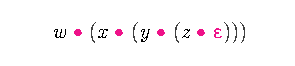
\includegraphics[draft=false,trim={25 10 25 10}]{../graphics/rhs-norm}};
      \node (rn) at ( 2, 2) {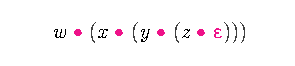
\includegraphics[draft=false,trim={25 10 25 10}]{../graphics/rhs-norm}};
      \node (la) at (-6, 0) {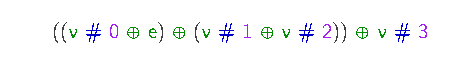
\includegraphics[draft=false,trim={25 10 22 10}]{../graphics/lhs-ast}};
      \node (ra) at ( 6, 0) {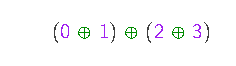
\includegraphics[draft=false,trim={25 10 48 10}]{../graphics/rhs-ast}};
      \node (le) at (-2,-2) {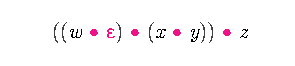
\includegraphics[draft=false,trim={25 10 23 10}]{../graphics/lhs-expr}};
      \node (re) at ( 2,-2) {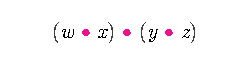
\includegraphics[draft=false,trim={25 10 20 10}]{../graphics/rhs-expr}};
      \draw[|-stealth] (la) to[out=90 , in=180] node[midway, fill=bg] {\AgdaFunction{⟦\_⇓⟧}} (ln);
      \draw[|-stealth] (la) to[out=270, in=180] node[midway, fill=bg] {\AgdaFunction{⟦\_⟧} } (le);
      \draw[|-stealth] (ra) to[out=90 , in=0  ] node[midway, fill=bg] {\AgdaFunction{⟦\_⇓⟧}} (rn);
      \draw[|-stealth] (ra) to[out=270, in=0  ] node[midway, fill=bg] {\AgdaFunction{⟦\_⟧} } (re);
      \foreach \e/\n in {le/ln,re/rn}
        \foreach \shft in {-0.6pt,0.6pt}
          \draw[AgdaField, transform canvas={xshift=\shft}, snake=coil, segment aspect=0, segment amplitude=0.4pt, segment length=4pt] (\e) -- (\n);
      \node[fill=bg] at (-2, 0) {\AgdaFunction{correct}};
      \node[fill=bg] at ( 2, 0) {\AgdaFunction{correct}};
      \foreach \shft in {-1.6pt, 0pt}
        \draw[AgdaDatatype, transform canvas={yshift=\shft}] (ln) -- (rn);
      \draw[AgdaDatatype, transform canvas={yshift=1.6pt}] (ln) -- (rn) node[midway, above] {\AgdaInductiveConstructor{refl}};
    \end{tikzpicture}
  }
\end{frame}
\begin{frame}
  \frametitle{Moving on to Polynomials}
  \note{
    We now know the components required for an automatic solver for some
    algebra: a canonical form, a concrete representation of expressions, and a
    proof of correctness. We now turn our focus to polynomials.

    The state-of-the art approach is presented in this paper.

    Also: choice of algebra.
  }
  \bibentry{gregoire_proving_2005}
\end{frame}
\begin{frame}
  \frametitle{Canonical Form}
  \note{
    The canonical representation of polynomials is a list of coefficients, least
    significant first (``Horner Normal Form''). Our initial attempt at encoding
    this representation is as follows.
  }
  \ExecuteMetaData[../Rings.tex]{dense-impl}
\end{frame} 
\begin{frame}
  \frametitle{Horner's Rule}
  \note<1>{
    Horner's rule is a method for evaluating polynomials which lets you avoid
    repeatedly exponentiating the input variable.
  }
  \begin{align*}
  p(x) &= a_0x^0 + a_1x^1 + a_2x^2 + ... a_nx^n \\
       &= a_0 + x(a_1 + x(a_2 + x (... a_n + x(0))))
  \end{align*}
  \pause
  \note<2>{
    Haskellers will recognize it as a foldr operation.
  }
  \ExecuteMetaData[../Rings.tex]{dense-eval}
\end{frame}
\begin{frame}
  \frametitle{Problems}
  \note<1>{As it stands, the above representation has two problems}
  \pause

  \note<2>{
    The representation suffers from the problem of trailing zeroes. In other
    words, the polynomial $2x$ could be represented by any of the following:

    This is a problem for a solver: the whole \emph{point} is that equivalent
    expressions are represented the same way. 
  }
  \begin{description}
  \item[Redundancy]
      \begin{align*}
        2x = \; & 0, 2 \\
                & 0, 2, 0 \\
                & 0, 2, 0, 0 \\
                & 0, 2, 0, 0, 0, 0, 0
      \end{align*}
      \pause
    \item[Inefficiency]
  \end{description}

  \note<3>{
    Expressions will tend to have large gaps, full only of zeroes. Something
    like $x^5$ will be represented as a list with 6 elements, only the last one
    being of interest. Since addition is linear in the length of the list, and
    multiplication quadratic, this is a major concern.
  }
\end{frame}
\begin{frame}[fragile]
  \frametitle{A Sparse Encoding}
  \note<1>{
    The solution usually used is a ``power index''. A representation of the gap
    between adjacent nonzero coefficients.

    We rewrite the following equation as so:
  }

  \(3 + 2x^2 + 4x^5 + 2x^7\) \pause \(= x^0 (3 + x x^1 (2 + x x^2 * (4 + x x^1 (2 + x 0))))\)
  \note<2>{
    And then we can represent it in a list like so:
  }

  \begin{minted}[autogobble]{Haskell}
    [(3,0),(2,1),(4,2),(2,1)]
  \end{minted}
\end{frame}
\begin{frame}
  \note{
    We actually go further than the previous approach, because we \emph{prove}
    that the coefficients are in normal form.
  }
  \ExecuteMetaData[../Rings.tex]{sparse-decl}
\end{frame}
\begin{frame}
  \frametitle{Termination}
  \note{
    Ever-present in Agda is the need to prove termination.

    Our conversion to normal form, and the operations on that normal form, are
    complex, and not trivially terminating.

    To pass the termination checker, a recursive call has to have structurally
    smaller arguments. In other words, the arguments must be subterms of what
    was given.

    Comparing these two recursive functions, only the first passes the
    termination checker. The first $n$ is a subterm of the argument passed in;
    in the second example, it's not.
  }
  \ExecuteMetaData[BasicTypes.tex]{fib}

  \ExecuteMetaData[BasicTypes.tex]{fib-nonterm}
\end{frame}
\begin{frame}
  \frametitle{Well-Founded Recursion}
  \note<1>{
    The majority of programs will be structurally recursive.

    However, some (as in the second fib above) will not be, and we will need
    some extra information to prove termination.

    In Agda, we do this using well-founded relations.

  }
  \note<2>{
    We don't add well-founded relations to the theory, as each individual
    relation may not be consistent with other notions of termination.

    Instead, for any relation, we \emph{reformulate} it in terms of structural
    recursion.
  }
  \only<1>{
    \begin{block}{Well-Founded Relation}
      Contains no infinite descending chains.

      ``Less than'' on $\mathbb{N}$

      \[ 1 < 2 < 4 < 8 \]
    \end{block}

    \bibentry{nordstrom_terminating_1987}

    Is this consistent?
  }
  \begin{onlyenv}<2>
    \ExecuteMetaData[BasicTypes.tex]{wellfounded}
  \end{onlyenv}
\end{frame}
\begin{frame}
  \frametitle{Homomorphism}
  \note{
    After termination is proven, we need to prove that the canonical form
    corresponds to the underlying carrier. This is proving that the operations
    we have defined are a ring homomorphism.

    The only last thing I'll mention is with regards to the nature of the
    proofs. They use a technique called the ``algebra of programming'' to
    shorten them up: because most of our functions are defined using
    higher-order folds and so on, we can express the proofs in very abstract,
    terse terms.

    The proofs are still roughly 1000 lines long, though.
  }
  \bibentry{bird_algebra_1997}

  \bibentry{mu_algebra_2009}
\end{frame}
\begin{frame}
  \frametitle{Interface}
  \note{
    Though what we have works, it's still awkward to use, because we ask the
    user to construct the AST themselves. This means they write the type twice,
    and it is often tedious to do so.

    This is the ``automatic'' proof for the monoid solver we had previously.
  }
  \ExecuteMetaData[../Monoids.tex]{ident-auto-proof}
\end{frame}
\begin{frame}[t, fragile]
  \vspace*{2.5cm}
  \adjustbox{width=1.15\linewidth, center}{
    \begin{tikzpicture}
      % \draw[help lines] (-8,-4) grid (8,3); 
      \node (ln) at (-2, 2) {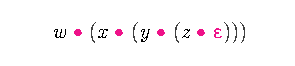
\includegraphics[draft=false,trim={25 10 25 10}]{../graphics/rhs-norm}};
      \node (rn) at ( 2, 2) {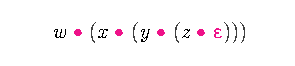
\includegraphics[draft=false,trim={25 10 25 10}]{../graphics/rhs-norm}};
      \node (la) at (-6, 0) {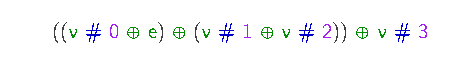
\includegraphics[draft=false,trim={25 10 22 10}]{../graphics/lhs-ast}};
      \node (ra) at ( 6, 0) {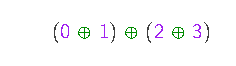
\includegraphics[draft=false,trim={25 10 48 10}]{../graphics/rhs-ast}};
      \node (le) at (-2,-2) {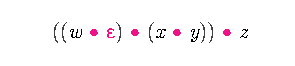
\includegraphics[draft=false,trim={25 10 23 10}]{../graphics/lhs-expr}};
      \node (re) at ( 2,-2) {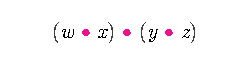
\includegraphics[draft=false,trim={25 10 20 10}]{../graphics/rhs-expr}};
      \draw[|-stealth] (la) to[out=90 , in=180] node[midway, fill=bg] {\AgdaFunction{⟦\_⇓⟧}} (ln);
      \draw[|-stealth] (la) to[out=270, in=180] node[midway, fill=bg] {\AgdaFunction{⟦\_⟧} } (le);
      \draw[|-stealth] (ra) to[out=90 , in=0  ] node[midway, fill=bg] {\AgdaFunction{⟦\_⇓⟧}} (rn);
      \draw[|-stealth] (ra) to[out=270, in=0  ] node[midway, fill=bg] {\AgdaFunction{⟦\_⟧} } (re);
      \foreach \e/\n in {le/ln,re/rn}
        \foreach \shft in {-0.6pt,0.6pt}
          \draw[AgdaField, transform canvas={xshift=\shft}, snake=coil, segment aspect=0, segment amplitude=0.4pt, segment length=4pt] (\e) -- (\n);
      \node[fill=bg] at (-2, 0) {\AgdaFunction{correct}};
      \node[fill=bg] at ( 2, 0) {\AgdaFunction{correct}};
      \foreach \shft in {-1.6pt, 0pt}
        \draw[AgdaDatatype, transform canvas={yshift=\shft}] (ln) -- (rn);
      \draw[AgdaDatatype, transform canvas={yshift=1.6pt}] (ln) -- (rn) node[midway, above] {\AgdaInductiveConstructor{refl}};
      \draw<2>[-angle 90, dashed] (re) to[out=270, in=270] node[near start, fill=bg] {\AgdaKeyword{quoteTerm}} ([shift={(1,0)}]ra.south);
      \draw<2>[-angle 90, dashed] (le) to[out=270, in=270] node[near start, fill=bg] {\AgdaKeyword{quoteTerm}} ([shift={(-1,0)}]la.south);
    \end{tikzpicture}
  }
  \note<1>{
    What we'd like to do is provide the ASTs here automatically, from the two
    expressions at the bottom.
  }
  \note<2>{
    What can we use for that? \emph{Reflection}

    Reflection is often thought to be the purview of unsafe or dynamic
    languages, but it actually fits really well into the dependently typed
    setting. As it happens, Agda has a decent (type-directed) macro system. The
    end result is a very clean system
  }
\end{frame}
\begin{frame}[standout]
  The Finished Solver
\end{frame}
\begin{frame}
  \note{
    Even more, because this relies on the \emph{type} of the hole (the inferred
    obligation) if you need to prove two things line up, you just pinpoint where
    they son't match, and say ``solve, please!''
  }
  \ExecuteMetaData[../ReflectDemo.tex]{refl-lemma}
\end{frame}
\begin{frame}[fragile]
  \frametitle{Setoids}
  \note<1>{
    We used a setoid throughout the solver, which really made things difficult
    for us.

    Usually, The purpose of this particular hair shirt is flexibility: users can
    still use the solver even if their type only satisfies the monoid laws
    modulo some equivalence relation (perhaps they are have an implementation of
    finite, mergeable sets as balanced trees, and want to treat two sets as
    equivalent if their elements are equal, even if their internal structures
    are not).

    It also frees up some very interesting applications, though.
  }
  \note<2>{
    All you need a setoid to be is something with symmetry, reflexivity, and
    transitivity. One example would be a list of rewrite rules! Now, the output
    is a proof, along with a \emph{step-by-step} solution to how you got from
    one equation to the other. We get wolfram alpha for free! And it's verified!

    Reflexivity is the empty list.

    Transitivity is concatenation.

    Symmetry is reverse.
  }
  \pause

  \only<2>{
    \begin{block}{Pedagogical Solutions}
      \ExecuteMetaData[BasicTypes.tex]{traced}
    \end{block}
  }

  \only<3>{
    \begin{block}{Isomorphisms}
      \ExecuteMetaData[BasicTypes.tex]{iso}
    \end{block}
  }
  \note<3>{
    Some of the type operations we mentioned earlier were ring-like: sum types,
    product types, the empty type, the singleton type, etc.

    Turns out these can be directly translated into polynomials!

    And the equivalence relation? An isomorphism! So now we can automatically
    construct isomorphisms between equivalent types.
  }
\end{frame}
\begin{frame}[fragile]
  \frametitle{The Correct-by-Construction Approach}
  \note<1>{
    The Agda and Coq communities exhibit something of a cultural difference when it
    comes to proving things. Coq users seem to prefer writing simpler, almost
    non-dependent code and algorithms, to separately prove properties about that
    code in auxiliary lemmas. Agda users, on the other hand, seem to prefer baking
    the properties into the definition of the types themselves, and writing the
    functions in such a way that they prove those properties as they go (the
    ``correct-by-construction'' approach).

    There are advantages and disadvantages to each approach. The Coq approach, for
    instance, allows you to reuse the same functions in different settings,
    verifying different properties about them depending on what's required. In Agda,
    this is more difficult: you usually need a new type for every invariant you
    maintain (lists, and then length-indexed lists, and then sorted lists, etc.). On
    the other hand, the proofs themselves often contain a lot of duplication of the
    logic in the implementation: in the Agda style, you avoid this duplication, by
    doing both at once. Also worth noting is that occasionally attempting to write a
    function that is correct by construction will lead to a much more elegant
    formulation of the original algorithm, or expose symmetries between the proof
    and implementation that would have been difficult to see otherwise.
  }
  \note<2>{
    The gregoire version as an example, is very much in the Coq style: the
    definition of the polynomial type has no type indices, and makes no requirements
    on its internal structure:

    The implementation presented here straddles both camps: we verify
    homomorphism in separate lemmas, but the type itself does carry information:
    it's indexed by the number of variables it contains, for instance, and it
    statically ensures it's always in canonical form. 
  }
  \begin{onlyenv}<2>
    \bibentry{gregoire_proving_2005}

    \begin{minted}[autogobble]{Coq}
      Inductive Pol (C:Set) : Set :=
        | Pc : C -> Pol C
        | Pinj : positive -> Pol C -> Pol C
        | PX : Pol C -> positive -> Pol C -> Pol C.
    \end{minted}
  \end{onlyenv} 

  \only<3>{\bibentry{geuvers_automatically_2017}}
  \note<3>{
    The correct-by-construction approach is explored in Idris, but they don't
    employ the same level of reflection or optimisation as we do.
  }
  \only<4>{\ExecuteMetaData[../Constr.tex]{constr-def}}
  \note<4>{
    Nonetheless, we do provide an implementation of this version, for
    comparison.
  }
\end{frame}
\begin{frame}[standout]
  Questions?
\end{frame}
\end{document}
